\chapter{A Mecânica dos Sólidos: tensão, deformação e deslocamento}

A Mecânica dos Sólidos é parte da física que estuda o comportamento de objetos sólidos sobre carregamentos, aplicando métodos analíticos para determinar suas características de resistência, rigidez e estabilidade. Seu conteúdo é notório por ser fundamental para grande parte da vida dos engenheiros, sendo mecânicos, civis ou mesmo eletricistas, ao lado de outras áreas também tão fundamentais, como Mecânica dos Fluidos e Termodinâmica. Sua aplicação é voltada ao projeto de estruturas a fim de que cumpram determinadas exigências, sejam tanto de deformação máxima, capacidade de carga e peso, como também de economia de materiais. E, por meio de ferramentas matemáticas, estuda os efeitos de tensão e deformação no interior de corpos sólidos. \cite{popov}

Este capítulo aborda os seguintes temas de Mecânica dos Sólidos, relevantes para o desenvolvimento inicial do módulo PHILLIPO.jl voltado à análise de estruturas elásticas sobre carregamentos contantes:
\begin{enumerate}
    \item tensão;
    \item deslocamento e deformação;
    \item estado de tensão;
    \item lei de Hooke generalizada;
    \item modelo de viga de Euler-Bernoulli;
    \item critérios de tensão máxima admissível.
\end{enumerate}

Todos os conceitos deste capítulo seguem as definições do livro de \citeauthor{popov}: \emph{Engineering Mechanics of Solids}, de 1990.

\section{Tensão}

Um corpo sólido se deforma quando submetido a carregamentos externos, distribuindo essas cargas ao longo de sua geometria. Tensão define a grandeza dessa distribuição agindo sobre áreas infinitesimais, de modo que qualquer secção do corpo revele forças internas que estejam em equilíbrio entre si, e que sejam balanceadas pelo carregamentos externos. \cite{popov}

Seja um corpo $\bm{K}$, sólido, em equilíbrio e de geometria qualquer, submetido a forças externas $\vec{F}$, a secção $S$ é um corte sobre esse corpo que revela as forças internas $\vec{P}$, conforme a figura \ref{fig:forcas_internas}.

\begin{figure}
    \centering
    \caption{Forças internas: seção em um sólido qualquer}
    \begin{subfigure}[b]{0.3\textwidth}
        \centering
        \begin{tikzpicture}[scale=0.6]
            \draw [->] (0,0,0) -- (4,0,0) node[anchor = west] {$z$};
            \draw [->] (0,0,0) -- (0,8,0) node[anchor = south] {$x$};
            \draw [->] (0,0,0) -- (0,0,4) node[anchor = east] {$y$};
        \end{tikzpicture}
        \caption{$y=x$}
        \label{fig:y equals x}
    \end{subfigure}
    \hfill
    \begin{subfigure}[b]{0.3\textwidth}
        \centering
        \begin{tikzpicture}[scale=0.6]
            \draw [->] (0,0,0) -- (4,0,0) node[anchor = west] {$x$};
            \draw [->] (0,0,0) -- (0,8,0) node[anchor = south] {$y$};
            \draw [->] (0,0,0) -- (0,0,4) node[anchor = east] {$z$};
            \shade[ball color = blue!60, opacity = 1] (0,4) circle (3cm);
            \draw[green] (-3,4) arc (180:360:3 and 0.6);
            \draw[dashed, green] (3,4) arc (0:180:-3 and 0.6);
            \begin{scope}[canvas is xz plane at y=4]
                \draw (-3,0) arc (0:360:-3); 
            \end{scope}
        \end{tikzpicture}
        \caption{$y=3\sin x$}
        \label{fig:three sin x}
    \end{subfigure}
    \hfill
    \begin{subfigure}[b]{0.3\textwidth}
        \centering
        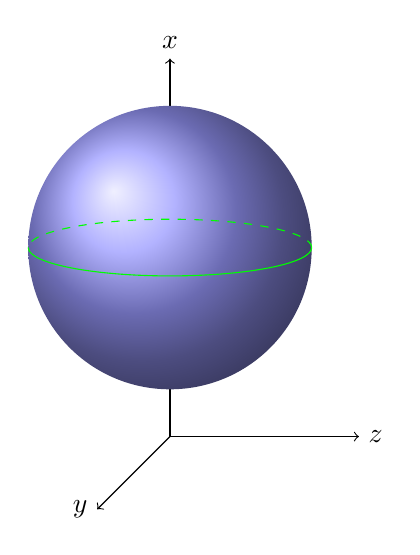
\begin{tikzpicture}[scale=0.6]
            \draw [->] (0,0,0) -- (4,0,0) node[anchor = west] {$z$};
            \draw [->] (0,0,0) -- (0,8,0) node[anchor = south] {$x$};
            \draw [->] (0,0,0) -- (0,0,4) node[anchor = east] {$y$};
            \shade[ball color = blue!40, opacity = 1] (0,4) circle (3cm);
            \draw[green] (-3,4) arc (180:360:3 and 0.6);
            \draw[dashed, green] (3,4) arc (0:180:3 and 0.6);
        \end{tikzpicture}
        \caption{$y=5/x$}
        \label{fig:five over x}
    \end{subfigure}
       \label{fig:forcas_internas}
\end{figure}